\chapter{Introdução}
\label{chap:introdução} 

\section{Contexto}

Segundo\cite{WillcocksTercerizacao} a terceirização do desenvolvimento de software é uma prática cada vez mais adotada por organizações. A terceirização de atividades, ou seja, o ato de transferir para fora da organização uma parte do seu processo produtivo não é uma prática recente. Atividades e processos que eram muito específicos dentro de uma organização foram transferidos, de forma parcial ou total, para outras organizações ou agentes externos \cite{leite_terceirizacao}.

Uma das motivações para a terceirização é a qualidade do serviço prometida pelas empresas fornecedoras. No entanto, existem vários riscos associados à decisão pela terceirização, que podem comprometer a qualidade esperada, como por exemplo: as expectativas de serviço e a resposta rápida não serem atendidas adequadamente; o serviço prestado apresentar qualidade inferior ao existente anteriormente; e as tecnologias utilizadas não corresponderem ao esperado\cite{WillcocksTercerizacao}. Segundo \citeonline{GuiaAquisicao} a aquisição de um \textit {software} é um processo complexo, principalmente no que diz respeito à caracterização dos requisitos necessários ao \textit {software} e às condições envolvidas na contratação como a qualidade esperada. 
 
Acompanhando o ritmo da terceirização o cenário com empresas terceirizadas contratadas para o desenvolvimento de \textit {software} está cada vez maior em organizações públicas. Tais organizações não são diretamente responsáveis pelo desenvolvimento do \textit {software} mas são responsáveis  pelo processo de verificação de sua qualidade conforme a norma \cite{Normativa4} que será explicada no capítulo \ref{chap:contratos} deste trabalho.


\section{Justificativa}

Segundo \cite{beck1999}\cite{fowler1999refactoring}, a qualidade de \textit{software} é medida pela qualidade de seu código-fonte. Conforme a \cite{ISO:15939}, medição é uma ferramenta primordial para avaliar a qualidade dos produtos e a capacidade de processos organizacionais, portanto, o Órgão Público contratante pode fazer uso do monitoramento de métricas de código-fonte para assistir ao processo de aferição de qualidade do \textit{software} desenvolvido pela contratada.

\citeonline{rego_monitoramento_2014} propôs uma solução automatizada para o monitoramento e interpretação de métricas de código-fonte com suporte de um ambiente de \textit{Data Warehousing}, que será explicada no Capítulo \ref{chap:arquitetura}. Este trabalho trata da evolução dessa solução, aplicada em uma Organização Pública Federal. Uma das principais contribuições deste trabalho foi a adição de: i)uma camada de visualização de métricas de código-fonte; ii) novos coletores de métricas de código-fonte. Estas adições  unificaram a visualização e interpretação de diferentes tipos de métricas de código-fonte em um mesmo ambiente.  


\section{Problema}
\label{problema} 

Com foco na avaliação de controles gerais de Tecnologia da Informação nos Órgãos públicos, em 2011, o Tribunal de Contas da União-TCU detectou, por meio de auditorias de governança de TI em diversos Órgãos, uma considerável frequência de irregularidades relacionadas à inexistência, deficiências e a falhas de processos de \textit{software} que comprometem a eficácia e eficiência das contratações de desenvolvimento de sistemas \cite{Acordao381_2011}. 

A inexistência de parâmetros de referência que para aferição da qualidade interna de código-fonte em contratações públicas expõe uma fragilidade nesse processo, decorrente da falta de uma metodologia que assegure a análise e interpretação dessas medidas. Os critérios indicados pelo TCU no acórdão \cite{Acordao381_2011} foram : Constituição Federal, art. 37, caput; Instrução Normativa 4/2008, SLTI/MPOG, art. 12, inciso II; Lei 8666/1993, art. 6º, inciso IX; Norma Técnica - ITGI - Cobit 4.1, PO8.3 - Padrões de desenvolvimento e de aquisições; Norma Técnica - NBR ISO/IEC - 12.207 e 15.504;e Resolução 90/2009, CNJ, art. 10. 

A auditoria do acordão \cite{Acordao381_2011} reforça o problema da falta de capacidade da administração pública em aferir a qualidade interna dos produtos de software desenvolvido por terceirizadas. Tendo esse problema  como motivação desta investigação científica, a questão geral de pesquisa deste trabalho é:

\textbf{O uso de um ambiente de \textit{Data Warehousing} para aferição da qualidade interna de software, apoiado por ferramentas de análise estática de código-fonte,  pode assistir ao processo de aferição da qualidade interna em uma organização pública federal?}


\section{Objetivos}

O objetivo geral deste trabalho é evoluir a solução proposta por \citeonline{paperrego} e utilizá-la para assistir ao processo de aferição de qualidade interna de um produto de software desenvolvido em um contrato de prestação de serviço para uma organização pública. Dentre os objetivos específicos deste trabalho estão:

\begin{easylist}[itemize]

& Adicionar à solução de \textit{DWing} a análise de erros e violações de código-fonte fornecidas por ferramentas já em uso na organização pública analisada, de forma a prover uma ambiente integrado e automatizado para análise, interpretação e visualização de dados de código-fonte;

& Construir uma camada de visualização de dados de forma a demonstrar as medidas e/ou suas interpretações, por meio de painéis informativos no ambiente de DWing.

& Analisar um sistema adquirido por um Orgão Púlico utilizando à solução de \textit{DWing} evoluída.

\end{easylist}

\section{Metodologia de pesquisa}

O que é uma pesquisa? De acordo com \cite{gil_como_2002} é o procedimento racional e sistemático que tem como objetivo proporcionar respostas aos problemas que são propostos. A pesquisa é requerida quando não se dispõe de informação suficiente para responder ao
problema, ou então quando a informação disponível se encontra em tal estado de desordem que não possa ser adequadamente relacionada ao problema.

Nessa seção, apresenta-se a metodologia de pesquisa adotada neste trabalho. Para
isso, foram definidos: a natureza da pesquisa; o tipo de metodologia de pesquisa; o tipo de abordagem de pesquisa; os métodos de procedimentos de pesquisa e os tipos de técnicas
de coletas de dados.

Os procedimentos de pesquisa selecionados foram pesquisa bibliográfica, documental, levantamento e estudo de caso. As técnicas de coleta de dados selecionadas foram
entrevistas, questionários e registro de observação na vida real. A seleção metodológica é apresentada na Figura \ref{7eixosqualidade} e a descrição das classificações adotadas se encontra nas Tabelas \ref{tab:descricaoMetodologia} e \ref{tab:descricaoMetodologia2}.

\begin{figure}[h!]
\centering
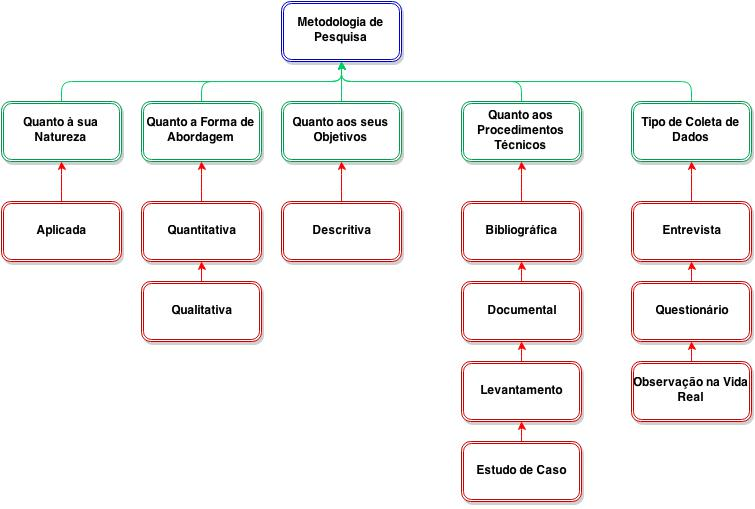
\includegraphics[keepaspectratio=false,scale=0.55]{figuras/figuras_nilton/selecaoMetodologica.png}
\caption{Metodologia de Pesquisa}
\label{7eixosqualidade}
\end{figure}

\begin{table}[!ht]
	\begin{center}
	
	\input{tabelas/tabelasNilton/tabelaDescricaoMetodologia1.ltx} 
	\caption{Descrição das classificações adotadas de pesquisa, conceitos extraídos de  \citeonline{metodologia_edna} parte 1.}
	\label{tab:descricaoMetodologia}
	\end{center}
	\end{table}	
	\FloatBarrier
	
	
	
	\begin{table}[!ht]
	\begin{center}
	
	\input{tabelas/tabelasNilton/tabelaDescricaoMetodologia2.ltx} 
	\caption{Descrição das classificações adotadas de pesquisa, conceitos extraídos de  \citeonline{metodologia_edna} parte 2.}
	\label{tab:descricaoMetodologia2}
	\end{center}
	\end{table}	
	\FloatBarrier

Segundo \cite{yin2001estudo}, o estudo de caso é um conjunto de procedimentos pré-especificados para se obter uma investigação empírica que investiga um fenômeno contemporâneo dentro de seu contexto da vida real, especialmente quando os limites entre o fenômeno e o contexto não estão claramente definidos. Uma grande vantagem do estudo de caso é a sua capacidade de lidar com uma ampla variedade de evidências - documentos, artefatos, entrevistas e observações - além do que pode estar disponível no estudo histórico convencional. Além disso, em algumas situações, como na observação participante, pode ocorrer manipulação informal.

\cite{wohlin2012experimentation} fraciona o estudo de caso em cinco passos. Nesta pesquisa, o estudo de caso compreende os passos: Planejar o Estudo de Caso; Coletar Dados; Analisar Dados Coletados e Compartilhar os Resultados. Portanto, os passos Projetar o Estudo de Caso e Preparar a Coleta de Dados definidas por \citeonline{wohlin2012experimentation} foram agrupadas no passo Planejar o estudo de caso como na Figura \ref{passo Estudo de Caso}.

\begin{figure}[h!]
\centering
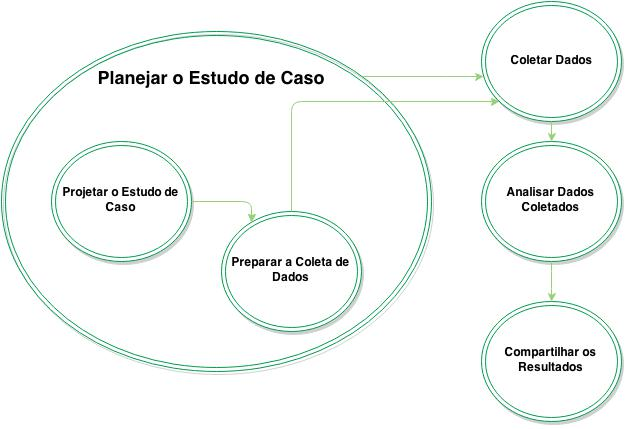
\includegraphics[keepaspectratio=false,scale=0.7]{figuras/figuras_nilton/passosEstudoCaso.png}
\caption{Passos do Estudo de Caso}
\label{passo Estudo de Caso}
\end{figure}

O passo Planejar o Estudo de Caso consiste na determinação do objetivo e da questão de pesquisa, da escolha da metodologia de pesquisa, da definição das fases da pesquisa, da definição do procedimentos de pesquisa, do protocolo, das técnicas de coleta de dados e da proposta do trabalho final.

No passo Coletar Dados são executados os procedimentos de pesquisa e as técnicas de coletas de dados a seguir:

\begin{easylist}[itemize]
& Pesquisa Bibliográfica: pesquisa realizada a partir de livros, dissertações e trabalhos relacionados à área de pesquisa;

& Pesquisa Documental: pesquisa realizada a partir de documentos publicados por organizações públicas;

& Estudo de Caso: utilizar um estudo de caso real de uma organização pública brasileira;

& Entrevistas: dados serão coletados por meio de entrevistas, além de questionário, para incremento do estudo de caso;

& Documentos: coleta de dados dos documentos dos processos fornecidos pelo Órgãos público do estudo de caso será realizada para coleta de dados para análise;

& Observação na Vida Real: coleta de dados a partir da observação dentro do Órgão Público;

\end{easylist}

O passo Analisar Dados Coletados é onde os dados coletados serão analisados e interpretados. A análise compreende tanto a análise quantitativa quanto a análise qualitativa.

Por fim, o passo Compartilhar os resultados diz respeito expor os resultados de forma adequada para o leitor alvo.

\section{Metodologia de Desenvolvimento}

A metodologia de desenvolvimento utilizada no Trabalho de Conclusão de Cursos 1 foi baseada em reuniões quinzenais junto ao orientador cujo objetivo era discutir sobre o tema, levantar as necessidades, atribuir atividades para suprir as necessidades e validar os resultados das atividades já realizadas. Ao final do Trabalho de Conclusão de Cursos 1 foi elaborado um cronograma com as macro atividades para serem realizadas durante a o Trabalho de Conclusão de Cursos 2. Contudo, após a defesa do Trabalho de Conclusão de Cursos 1, houve um realinhmanento sobre os objetivos esperados, o que ressultou a adequação do planejamento inicial.

Objetivando maximizar a produtividade, as reuniões passaram a ser semanais e passamos a utilizar a ferramenta \textit{kanbanFlow} para gerir tarefas usando o método \textit{Kanban}. O \textit{Kanban} foi dividido em 4 colunas como mostra a Figura \ref{kanban} :

\begin{easylist}[itemize]

& \textbf{Main Backlog:} Onde ficam todas as atividades que devem ser realizadas durante todo o Trabalho de Conclusão de Cursos 2. 

& \textbf{Sprint Backlog:} Onde ficam as atividades que devem ser realizadas durante a semana(\textit{Sprint}).

& \textbf{In Progress:} Onde ficam as atividades que estão em andamento. 

& \textbf{Done:} Onde ficam as atividades finalizadas.

\end{easylist}

\begin{figure}[h!]
\centering
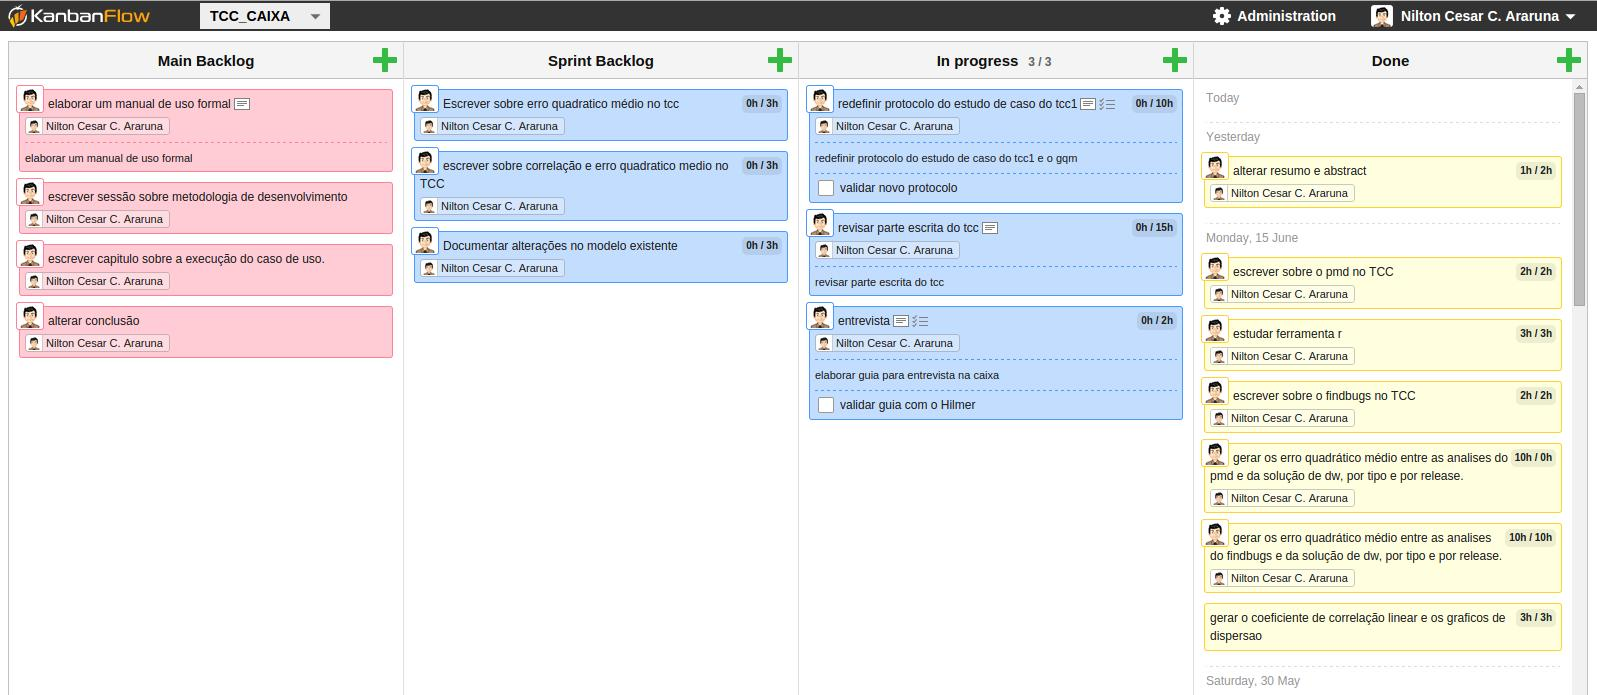
\includegraphics[keepaspectratio=false,scale=0.3]{figuras/figuras_nilton/kanban.png}
\caption{Estrutura do \textit{Kanban}.}
\label{kanban}
\end{figure}

O Apêndice \ref{sec:kanban} contém um relatório que demonstra as atividades realizadas durante todo o Trabalho de Conclusão de Cursos 2 e as horas gastas por atividade divididas pelas colunas descritas acima.


\section{Organização do Trabalho}

Esse trabalho está dividido em 6 capítulos:

	\begin{easylist}[itemize]	
	

	& \textbf{Capítulo 2 - Métricas de Software:} Capítulo responsável pela explicação teórica a respeito do que são métricas de código e verificadores de erros e como elas foram utilizadas no desenvolvimento da solução que esse trabalho busca analisar.
	
	& \textbf{Capítulo 3 - Contratações de Fornecedores de Desenvolvimento de Software:} Capítulo responsável por introduzir as principais informações referentes à Contratação de Fornecedores de Desenvolvimento de Software. Para isso, o capítulo é iniciado com uma visão geral sobre a importância das contratações e suas principais características. Posteriormente, é apresentado um resumo da Instrução Normativa 04.
	
	& \textbf{Capítulo 4 - Data Warehouse:} Nesse capítulo, serão apresentados conceitos teóricos sobre \textit{Data Warehousing}, assim como a maneira como foi desenvolvido e como funciona o ambiente de \textit{Data Warehouse} para armazenamento de métricas de código fonte. Também trata a importância da visualização dos dados e quais as ferramentas foram utilizadas para a implantação do \textit{dashboard}.
	
	& \textbf{Capítulo 5 - Estudo de Caso:} É apresentado o projeto do estudo de caso resultante do passo planejar Estudo de Caso, buscando demonstrar o escopo e elaborar um protocolo para o estudo de caso realizado. Elementos de pesquisa foram identificados e explicados, como o problema a ser resolvido, os objetivos a serem alcançados no estudo de caso, quais os métodos de coleta, sua execução e a análise dos dados.
	
	& \textbf{Capítulo 6 - Conclusão:} Capítulo responsável por apresentar as conclusões, limitações do trabalho e trabalhos futuros.

	\end{easylist}
